%%%%% Projekt z předmětu IEL %%%% 
%% Autor: (Ivan Onufriienko, xonufr00)

\documentclass[]{fitiel} % dokumenty v češtině, implicitní
\usepackage{circuitikz}
\usepackage{siunitx}
\usepackage{subcaption}
\usepackage{amsmath}

% Pomocné funkce k popisu obvodu
\newcommand{\R}[1]{R\textsubscript{#1}}
\newcommand{\Uu}[1]{U\textsubscript{#1}}
\newcommand{\I}[1]{I\textsubscript{#1}}
\newcommand{\Gg}[1]{G\textsubscript{#1}}
\newcommand{\Cc}[1]{C\textsubscript{#1}}
\newcommand{\Ll}[1]{L\textsubscript{#1}}
\newcommand{\Z}[1]{Z\textsubscript{#1}}
% hlavička 
% příkaz logo - vkládá logo fakulty dle zvoleného jazyka
\title{\logo\\IEL -- protokol k projektu}
\author{Ivan Onufriienko \\ xonufr00}
\date{\today} % today - dnešní datum

\begin{document}
	\maketitle
	
	\tableofcontents
	
	\newpage
	
	%% vložení jednotlivých příkladů
	\section{Příklad 1}
% Jako parametr zadejte skupinu (A-H)
\prvniZadani{H}
\subsection{Výpočet $R_{ekv}$}
\begin{figure}[H]
     \centering
     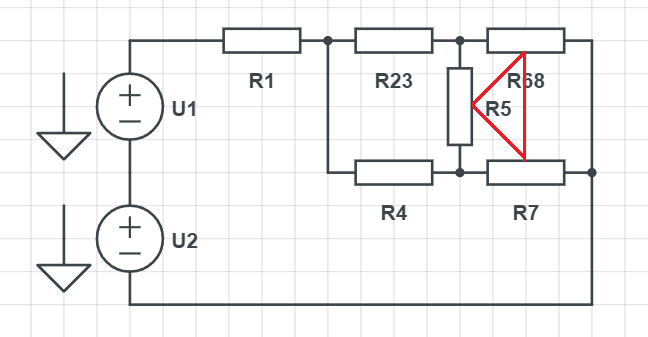
\includegraphics[scale=0.6]{pic1/u1o1.png}
     \caption{$R_2 + R_3$}
     \label{fig:Paralel_resistor_R23}
     \begin{quote}
     \centering
     $R_{23} =  \dfrac{R_2 * R_3}{R_2 + R_3} $  \\~\\
     $R_{23} =  \dfrac{600\Omega * 260\Omega}{600\Omega + 260\Omega} = 
     \dfrac{156000\Omega}{860\Omega} = 181.3953\Omega$ \\~\\
     $R_{68} =  {R_6 + R_8} $  \\~\\
     $R_{68} =  {870\Omega + 265\Omega} = {1135\Omega} $\\~\\
\end{quote}
\end{figure}
\begin{figure}[H]
    \centering
    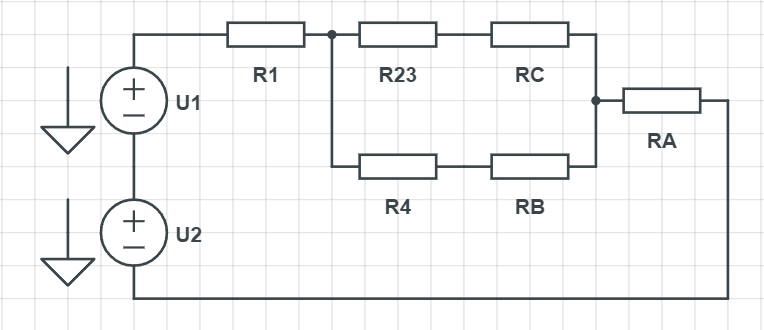
\includegraphics[scale=0.6]{pic1/u1o2.png}
    \caption{$Trojuhelnik \quad hvezda$}
    \label{fig:Trojuhelnik_Hvezda}
    \begin{quote}
    \centering
    $R_A =  \dfrac{R_{68} * R_7}{R_5 + R_{68} + R_7} $  \\~\\
    $R_B =  \dfrac{R_7 * R_5}{R_5 + R_{68} + R_7} $  \\~\\
    $R_C =  \dfrac{R_5 * R_{68}}{R_5 + R_{68} + R_7} $  \\~\\
    \medskip
    $R_A =  \dfrac{1135\Omega * 355\Omega}{575\Omega + 1135\Omega + 355\Omega} = \dfrac{402925\Omega}{2065\Omega} = 195.1210\Omega$ \\~\\
    $R_B =  \dfrac{355\Omega * 575\Omega}{575\Omega + 1135\Omega + 355\Omega} = \dfrac{204125\Omega}{2065\Omega} = 98.8498\Omega$ \\~\\
    $R_C =  \dfrac{575\Omega * 1135\Omega}{575\Omega + 1135\Omega + 355\Omega} = \dfrac{652625\Omega}{2065\Omega} = 316.0411\Omega$ \\~\\
    \end{quote}

    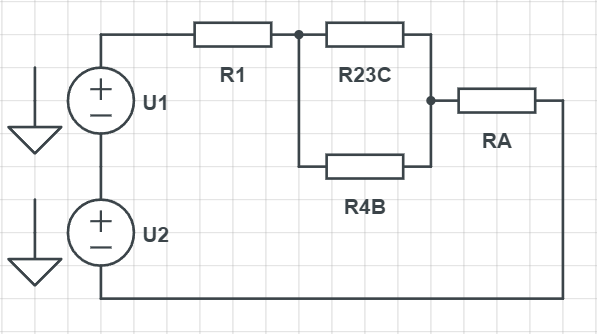
\includegraphics[scale=0.6]{pic1/u1o3.png}
    \caption{$Seriove \: zapojeni \quad R_{23} + R_C \quad a \quad R_4 + R_B $ }
    \label{fig:Serial_resistor_R23C_and_R4B}
    \begin{quote}
    \centering
    $R_{23C} = R_{23} + R_C $  \\~\\
    $R_{4B} = R_4 + R_B $  \\~\\
    $R_{23C} = 181.3953\Omega + 316.0411\Omega = 497.4364\Omega$ \\~\\
    $R_{4B} =310\Omega + 98.8498\Omega = 408.8498\Omega$ \\~\\
    \end{quote}
\end{figure}
\begin{figure}[H]
     \centering
     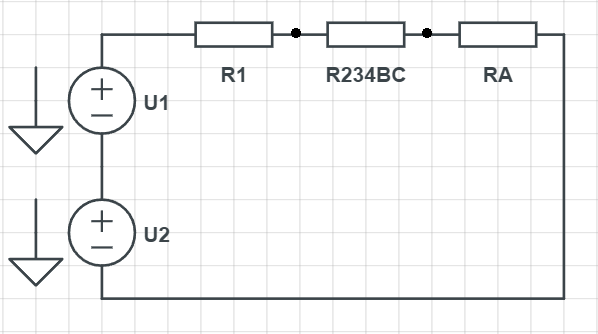
\includegraphics[scale=0.6]{pic1/u1o4.png}
     \caption{$Paralelne \: zapojene \: R_{23C} \: a \: R_{4B} \: a \: Zjednoduseni \: do \: R_{ekv}$}
     \label{fig:Paralel_resistor_R234BC}
     \begin{quote}
     \centering
     $R_{234BC} =  \dfrac{R_23C * R_4B}{R_23C + R_4B} $  \\~\\
     $R_{234BC} =  \dfrac{497.4364\Omega * 408.8498\Omega}{497.4364\Omega + 408.8498\Omega} = 
     \dfrac{203376.7726\Omega}{906.2862\Omega} = 224.4067\Omega$ \\~\\
\end{quote}
    \label{fig:REKV}
    \begin{quote}
    \centering
    $R_{ekv} = R_{1234ABC} = R_1 + R_{234BC} + R_A$  \\~\\
    $R_{ekv} = R_{1234ABC} = 680\Omega + 224.4067\Omega + 195.1210\Omega = 1099.5279 \Omega $  \\
    \end{quote}
    S $R_{ekv}$ nyní můžeme vypočítat celkový proud v obvodu Ohmovým zákonem: $I = \dfrac{U}{R_{ekv}}$
    \begin{quote}
    \centering
    $U = U_1 + U_2$ \\~\\
    $U = 135\Vo + 80\Vo = 215\Vo$ \\~\\
    $I = \dfrac{215\Vo}{1099.5279\Omega} = 0.0266\Am$
    \end{quote}
\end{figure}
    \subsection{Výpočet $U_{R2}$}
    \begin{quote}
    \centering
	Rozložíme zpětně obvod \\~\\
	$U_{R234BC} = I * R_{234BC}$ \\~\\
	$U_{R234BC} = 0.0266\Am * 224.4067\Omega = 43.8801\Vo$ \\~\\
    \end{quote}




\begin{figure}[H]
    \centering
    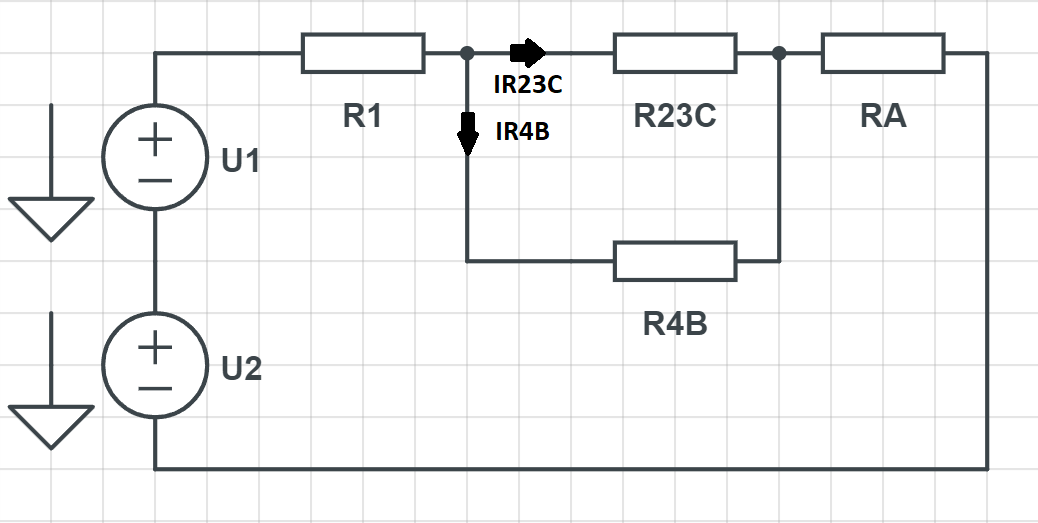
\includegraphics[scale=0.45]{pic1/u1o5.png}
    \begin{quote}
    \centering
    $I_{R23C} = \dfrac{U_{R2346BC}}{R_{23C}} $ \\~\\
	$I_{R23C} = \dfrac{43.8801\Vo}{497.4364\Omega} = 0.0882\Am $ \\~\\
    \end{quote}
\end{figure}
\begin{figure}[H]
    \centering
    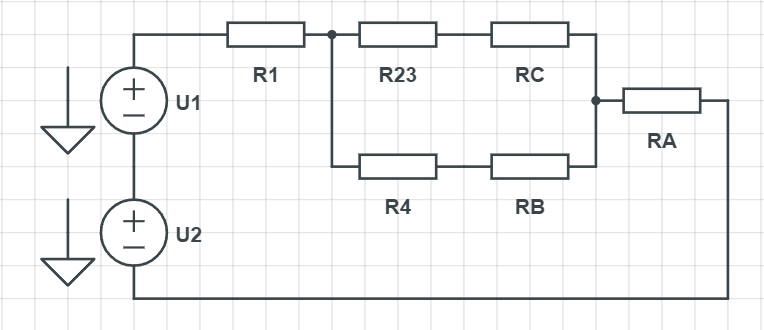
\includegraphics[scale=0.6]{pic1/u1o6 .png}
    \begin{quote}
    \centering
    $I_{R23} = I_{R23C}$ \\~\\
	$U_{R23} = I_{R23}*R_{23} $ \\~\\
	$U_{R23} = 0.0882\Am * 181.3953\Omega = 16.0016\Vo $ \\~\\
    \end{quote}
\end{figure}
\begin{figure}[H]
    \centering
    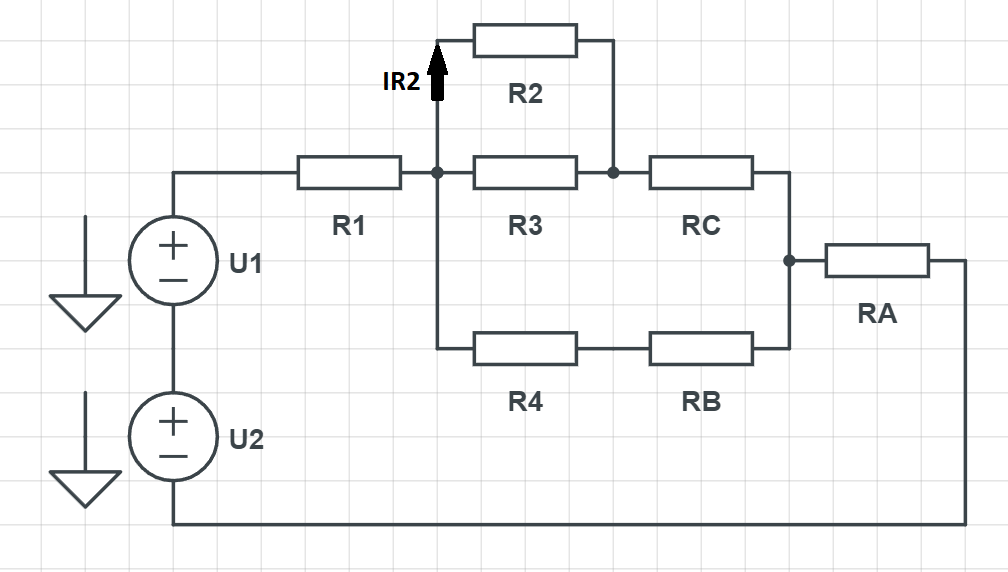
\includegraphics[scale=0.45]{pic1/u1o7.png}
    \begin{quote}
        \centering
         $U_{2} = U_{23} = 16.0016\Vo $ \\~\\
         $I_{R2} = \dfrac{U_{R23}}{R_{2}}$ \\~\\
         $I_{R2} = \dfrac{16.0016\Vo}{600\Omega} = 0.0266\Am$ \\~\\
    \end{quote}
\end{figure}
 \newpage
	\section{Příklad 2}
% Jako parametr zadejte skupinu (A-H)
\druhyZadani{G}
\subsection{Výpočet Re}
\begin{figure}[H]
    \centering
    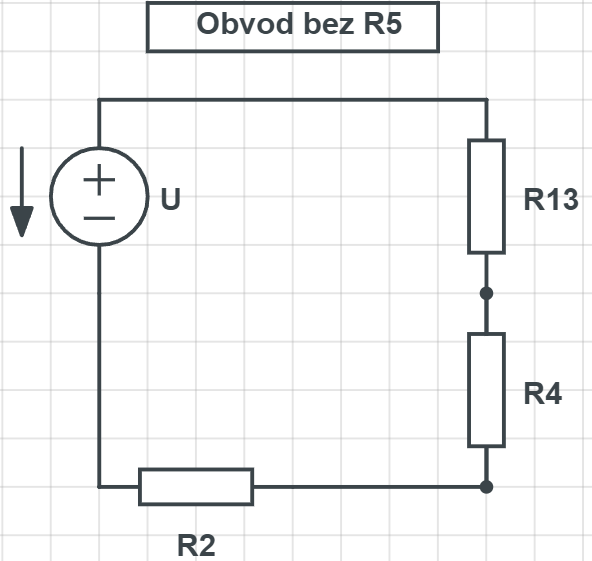
\includegraphics[scale=0.5]{pic2/u2o1.png}
    \caption{Seriove zapojeni $R_1 \: a \: R_3$}
    \label{fig:Serial_resistor_R13}
    \begin{quote}
    \centering
    $R_{13} = R_1 + R_3$ \\~\\
    $R_{13} = 250\Omega + 615\Omega = 865\Omega$
    \end{quote}
\end{figure}
\begin{figure}[H]
    \centering
    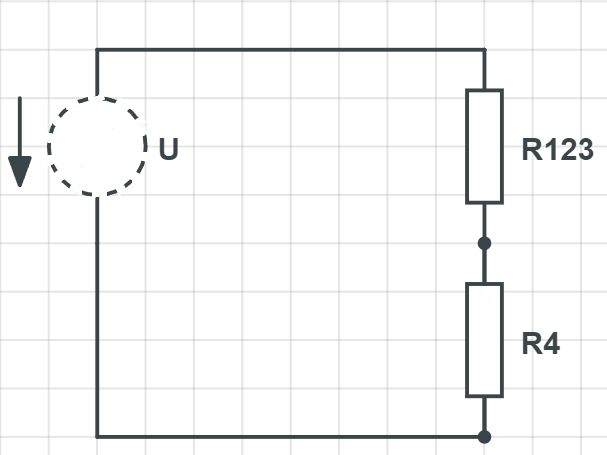
\includegraphics[scale=0.5]{pic2/u2o2.png}
    \caption{Seriove zapojeni $R_{13} \: a \: R_2$}
    \label{fig:Paralel_resistor_R123}
    \begin{quote}
    \centering
    $R_{345} = R_{13} + R_2$ \\~\\~\\
    $R_{345} = 865\Omega + 250\Omega = 1180\Omega$
    \end{quote}
\end{figure}

\begin{figure}[H]
    \centering
    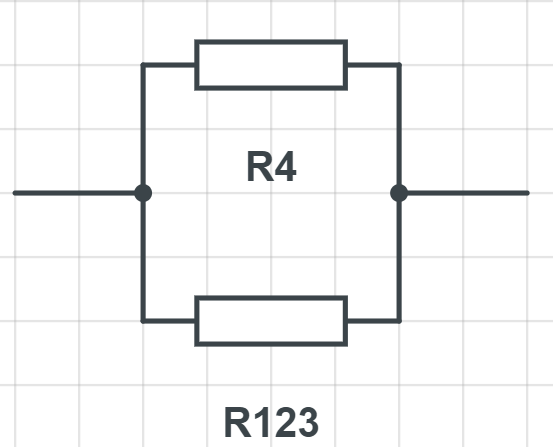
\includegraphics[scale=0.5]{pic2/u2o3.png}
    \caption{Paralelne zapojeni $R_{123} \: a \: R_4$}
    \label{fig:Paralel_resistor_R1234}
    \begin{quote}
    \centering
    $R_e = R_{1234} = \dfrac{R_{123} * R_4}{R_{123} + R_4}$ \\~\\~\\
    $R_e = \dfrac{1180\Omega * 180\Omega}{1180\Omega + 180\Omega} = \dfrac{212 400\Omega}{1360\Omega} = 156.1764\Omega$
    \end{quote}
\end{figure}
\subsection{Výpočet Ue}

\begin{figure}[H]
    \centering
    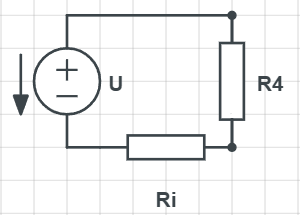
\includegraphics[scale=0.9]{pic2/u2o3.5.png}
    \begin{quote}
        \centering
	    Vypočítáme pomocí napětoví děliče \\~\\ 
	    $U_e = U * \dfrac{R_4}{R_4 + R_{123}} $ \\~\\
	    $U_e = 180\Vo * \dfrac{180\Omega}{180\Omega + 1180\Omega}  = 
	    180\Vo * \dfrac{180\Omega}{1360\Omega} = 23.8235\Vo$ \\~\\
	   
    \end{quote}
\end{figure}

\subsection{Výpočet $U_{R5} \: a \: I_{R5}$}

\begin{figure}[H]
    \centering
    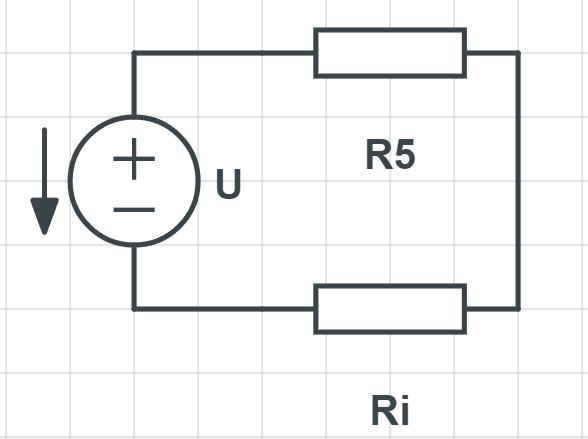
\includegraphics[scale=0.5]{pic2/u2o4.png}
    \begin{quote}
        \centering
	   $I_{R5} = \dfrac{U_e}{R_5 + R_e} = \dfrac{23.8235\Vo}{460\Omega + 156.1764\Omega}
	   = \dfrac{23.8235\Vo}{616.1764\Omega} = 0.0386635\Am$ \\~\\
	   $U_{R5} = R_5 * I_{R5} = 460\Omega * 0.0386635\Am = 17.7852\Vo$
    \end{quote}
\end{figure} \newpage
	\section{Příklad 3}
% Jako parametr zadejte skupinu (A-H)
\tretiZadani{H}
\begin{figure}[H]
    \centering
    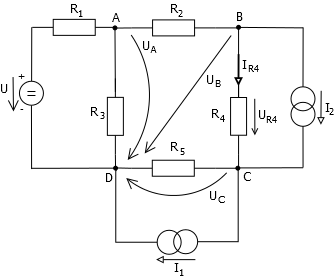
\includegraphics[scale=0.8]{pic3/Pr3_2022.png}
    \begin{quote}
        \centering
	   $\phi D = 0$ \\~\\
	   $I_{R1} - I_{R3} - I_{R2}  = 0$ \\
	   $I_{R2} - I_{R4} - I_2 = 0$ \\
	   $I_{R4} + I_2 - I_{R5} - I_1 = 0$ \\
    \end{quote}
\end{figure}
\newpage
\begin{quote}
    \centering
    $I_{R1} = \dfrac{(\phi D - \phi A + U)}{R_1} = \dfrac{U - \phi A}{R_1} $ \\~\\
    $I_{R2} = \dfrac{(\phi A - \phi B)}{R_2} $ \\~\\
    $I_{R3} = \dfrac{(\phi A - \phi D)}{R_3} = \dfrac{\phi A}{R_3}$ \\~\\
    $I_{R4} = \dfrac{(\phi B - \phi C)}{R_4} $ \\~\\
    $I_{R5} = \dfrac{(\phi C - \phi D )}{R_5} = \dfrac{\phi C}{R_5} $ \\~\\ 
\end{quote}
\begin{quote}
    \medskip
    \medskip
    \centering
    $\dfrac{U}{R_1} - \dfrac{\phi A}{R_1} -  \dfrac{\phi A}{R_3} - \dfrac{\phi A}{R_2} + \dfrac{\phi B}{R_2} = 0$ \\~\\ 
    $\dfrac{\phi A}{R_2} -  \dfrac{\phi B}{R_2} - \dfrac{\phi B}{R_4} + \dfrac{\phi C}{R_4} - I_2 = 0$ \\~\\ 
    $\dfrac{\phi B}{R_4} - \dfrac{\phi C}{R_4} + I_2 - \dfrac{\phi C}{R_5} - I_1 = 0$ \\~\\ 
\end{quote}
\begin{quote}
    \medskip
    \medskip
    \centering
    $-\phi A * (\dfrac{1}{R_1} +  \dfrac{1}{R_2} + \dfrac{1}{R_3}) + \phi B * (\dfrac{ 1}{R_2} )  = -\dfrac{U}{R_1}$ \\~\\ 
    $\phi A * (\dfrac{1}{R_2}) - \phi B * (\dfrac{1}{R_2} + \dfrac{1}{R_4} ) + \phi C * (\dfrac{1}{R_4})  = I_2 $ \\~\\
    $\phi B * (\dfrac{1}{R_4}) - \phi C * (\dfrac{1}{R_4} + \dfrac{1}{R_5})  = I_1 - I_2 $ \\~\\
\end{quote}
\begin{align*}
	\begin{pmatrix}
		-(\dfrac{1}{47}+\dfrac{1}{39}+\dfrac{1}{58})&\dfrac{1}{39}&0\\
		\dfrac{1}{39}&-(\dfrac{1}{39}+\dfrac{1}{28})&\dfrac{1}{28}\\
		0&\dfrac{1}{28}&-(\dfrac{1}{28}+\dfrac{1}{25})
	\end{pmatrix}\times
	\begin{pmatrix}
		\phi A\\
		\phi B\\
		\phi C
	\end{pmatrix}=
	\begin{pmatrix}
		-\dfrac{130}{47}\\
		0.5 \\
		0.45
	\end{pmatrix} \\
	\begin{pmatrix}
		\phi A\\
		\phi B\\
		\phi C
	\end{pmatrix}=
	\begin{pmatrix}
		-20,2480& -11,6646& -5,5022\\
		-11,6646& -29,1872& -13,7676\\
		-5,5022& -13,7676& -19,7017
	\end{pmatrix}\times
	\begin{pmatrix}
		-\dfrac{130}{47}\\
		0.5 \\
		0.45
	\end{pmatrix}
\end{align*}

\begin{quote}
    \centering
    $\phi A = 47.6969 \Vo$ \\ 
    $\phi B = 11.4748 \Vo$ \\
    $\phi C = -0.5307 \Vo$ \\ 
    \medskip
    \medskip
    $I_{R4} = \dfrac{(\phi B - \phi C)}{R_4} = \dfrac{( 11.4748\Vo + 0.5307 \Vo)}{28\Omega} = 0.4287\Am$ \\~\\
    $U_{R4} = \phi B - \phi C = 11.4748 \Vo + 0.5307 \Vo = 12.006\Vo$
\end{quote}
  \newpage
	\section{Příklad 4}
% Jako parametr zadejte skupinu (A-H)
\ctvrtyZadani{H}
\begin{figure}[H]
    \centering
    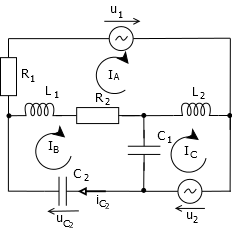
\includegraphics[scale=0.8]{pic4/Pr4_2022.png}
    \caption{Smyčkové proudy}
\end{figure}
U střídavého napětí využijeme stejné ohmovy zákony jako jsme využívali dosud. Jen s rozdílem, že nám zde přibyli impedance nelineárních součástek. Pro metodu smyčkových využijeme matici podobně jako v příkladu 3 jen se změnou, že nyní počítáme proudy smyček narozdíl od uzlových napětí.

Impedance pro cívku a kondenzátor spočteme následovně:
\begin{align*}
	\omega &= 2\pi f \\
	\Z{C} &= \frac{-j}{\omega C}\\
	\Z{L} &=  j\omega L
\end{align*}

\begin{align*}
	\I{A}:\quad&\Uu{1} + \Uu{R1} + \Uu{L2} + \Uu{R2} + \Uu{L1}  = 0\\
	\I{B}:\quad&\Uu{L1} + \Uu{R2} + \Uu{C2} + \Uu{C1} = 0 \\
	\I{C}:\quad&\Uu{L2} + \Uu{2} + \Uu{C1}  = 0
\end{align*}

\begin{align*}
	\I{A}:\quad&\I{A}(\Z{L1}+\Z{L2}+\R{1}+\R{2}) - \I{B}(\Z{L1}+\R{2}) - \I{C}\Z{L2} = -\Uu{1} \\
	\I{B}:\quad&-\I{A}(\Z{L1} + \R{2}) + \I{B}(\R{2}+\Z{L1}+\Z{C1}+\Z{C2})-\I{C}\Z{C1} = 0 \\
	\I{C}:\quad&-\I{A}\Z{L2} - \I{B}\Z{C1} + \I{C}(\Z{C1}+\Z{L2}) = -\Uu{2}
\end{align*}

Matice pro proudové smyčky:
	
\begin{align*}
	\begin{pmatrix}
		Z_{L2}+Z_{L1}+R_1+R_2&-Z_{L1}-R_2&-Z_{L2}\\ 
		-Z_{L1}-R_2&R_2+Z_{L1}+Z_{C1}+Z_{C2}&-Z_{C1}\\ 
		-Z_{L2}&-Z_{C1}&Z_{C1}+Z_{L2}
	\end{pmatrix}
	\times
	\begin{pmatrix}
		I_A\\ I_B\\ I_C
	\end{pmatrix}
	=
	\begin{pmatrix}
		-U_1\\ 0\\ -U_2
	\end{pmatrix}
\end{align*}

\subsection{Výpočet napětí a fázového posunu \Ll{2}}
Pro výpočet \Uu{C2} využijeme Ohmův zákon. Nesmíme zapomenout že se zde pracujeme s množinou imaginárních čísel, takže pro náš výsledek musíme využít vzorec pro absolutní hodnotu imaginárního čísla:

\begin{align*}
	\Uu{C2} &= \I{B}\times j\omega \Cc{2} \\
	\Uu{C2}| &= \sqrt{Re(\Uu{C2})^2 + Im(\Uu{C2})^2}
\end{align*}

Fázový posun vypočítáme jako arkus tangens, kde x je reálná část imaginárního čísla a y je imaginární část imaginárního čísla.

\begin{align*}
	\varphi_{C2}&= arctan(\frac{Im(\Uu{C2})}{Re(\Uu{C2})})
\end{align*}

\subsection{Dosazení}
Impedance:

\begin{align*}
	\omega &= 2\pi f \\
	\Z{C1} &= \frac{-j}{\omega \Cc{1}}\\
	\Z{C2} &= \frac{-j}{\omega \Cc{2}}\\
	\Z{L1} &=  j\omega \Ll{1} \\
	\Z{L2} &=  j\omega \Ll{2}
\end{align*}


\begin{align*}
\begin{pmatrix}20+95.5016*j+44.766375*j	&-10-95.5016*j&-44.766375*j\\ 
-10-95.5016*j&10+95.5016*j-10.8088*j-23.93378*j&10.8088*j\\ 
-44.766375*j&10.8088*j&44.766375*j-10.8088*j
\end{pmatrix}
\begin{pmatrix}I_A\\ 
I_B\\ 
I_C
\end{pmatrix}
=
\begin{pmatrix}
-5\\ 
0\\ 
-6
\end{pmatrix}
\end{align*}

\begin{align*}
	\I{A} &= (-0,0979-0,27j)\ \si{\ampere} \\
	\I{B} &= (-0,1128-0,4187j)\ \si{\ampere} \\
	\I{C} &= (-0,0931-0,046j)\ \si{\ampere}
\end{align*}

\begin{align*}
	\I{C2} &= \I{B} = (-0,1128-0,4187j)\ \si{\ampere} \\
	\Uu{C2} &= \I{C2} \times \Z{C2} = (-10,02107+2,69973j)\ \si{\volt} \\
	\varphi_{C2}&= \arctan(\frac{Im(\Uu{C2})}{Re(\Uu{C2})}) = \arctan\frac{2,69973}{-10,37837} =-0,254491 rad = 165,41874^\circ \\
	|\Uu{C2}| &= \sqrt{Re(\Uu{C2})^2 + Im(\Uu{C2})^2} = \sqrt{(-10,02107)^2+2,69973^2} = 10,37837\ \si{\volt}
\end{align*} \newpage
	\section{Příklad 5}
% Jako parametr zadejte skupinu (A-H)
\patyZadani{G}

\subsection{Řešení: Sestavení diferenciální rovnice}

Sestavíme rovnici pro proud na cívce i\textsubscript{L}:
\begin{align*}
	i'_L &= \frac{U_L}{L}
\end{align*}

Napětí na cívce si můžeme vyjádřit za pomocí 2. Kirchhoffova zákona:

\begin{align*}
	U &= U_R + U_L\\
	U_L &= U-U_R
\end{align*}

Vzniklou diferenciální rovnici upravíme:

\begin{align*}
	i'_L &= \frac{U-U_R}{L} \\
	i'_L &= \frac{U-Ri_L}{L} \\
	Li'_L + Ri_L &= U
\end{align*}

Dosadíme naše hodnoty:

\begin{align*}
	50i'_L + 25i_L &= 10
\end{align*}

Podívejme se na obecný tvar pro cívku, jestli už máme co potřebujeme:

\begin{align*}
	i_L(t)=K(t)\times e^{\lambda t}
\end{align*}

Chybí nám $\lambda$ a $K(t)$, tak ty proměnné musíme najít a vypočítat.

\begin{figure}[H]
Vzhledem k tomu, že neznáme $\lambda$ ani K(t), tak si je musíme spočítat, začneme s $\lambda$:

\begin{align*}
	50\lambda + 25 &= 0 \\
	\lambda &= - \frac{25}{50} \\
	\lambda &= -\frac{1}{2}
\end{align*}
\end{figure}

Nyní můžeme $\lambda$ dosadit do obecného tvaru, který pak zderivujeme, abychom měli diferenciální tvar rovnice naší cívky, pro dosazení do rovnice která nám vyšla předtím.

Nejprve tedy obecný tvar a jeho derivace:
\begin{align*}
	i_L(t) &= K(t)\times e^{\lambda t}\\
	i_L(t) &= K(t)\times e^{-\frac{1}{2}t} \\
	i_L(t)'&= K(t)'\times e^{-\frac{1}{2}t} - \frac{1}{2}K(t)e^{-\frac{1}{2}t}
\end{align*}

Nyní můžeme tedy dosadit do naší diferenciální rovnice:
\begin{align*}
	50(K(t)&'\times e^{-\frac{1}{2}t} - \frac{1}{2}K(t) \times e^{-\frac{1}{2}t}) + 25(K(t)\times e^{-\frac{1}{2}t}) = 10 \\
	50K(t)'&\times e^{-\frac{1}{2}t} - 25K(t)\times e^{-\frac{1}{2}t} + 25K(t)\times e^{-\frac{1}{2}t} = 10 \\
	50K(t)'&\times e^{-\frac{1}{2}t} = 10 \\
	K(t)'&\times e^{-\frac{1}{2}t} = \frac{10}{50} \\
	K(t)'&\times e^{-\frac{1}{2}t} = \frac{1}{5} \\
	K(t)'& = \frac{1}{5}\times e^{\frac{1}{2}t}
\end{align*}

Máme $K(t)$. Teda skoro máme, v obecném tvaru to není derivace, takže to musíme ještě zintegrovat:

\begin{align*}
	K(t) &= \int \frac{1}{5}\times e^{\frac{1}{2}t} dt \\
	K(t) &= \frac{2}{5} e^{\frac{1}{2}t} + C
\end{align*}

Nyní už máme co potřebujeme, tak dosadíme do analytické rovnice a pak provedeme kontrolu:
\begin{align*}
	i_L(t) &= K(t) \times e^{\lambda t} \\
	i_L(t) &= (\frac{2}{5} e^{\frac{1}{2}t} + C) \times e^{-\frac{1}{2} t} \\
	i_L(t) &= \frac{2}{5} + C \times e^{-\frac{1}{2} t}
\end{align*}

Nyní si vypočítáme C dle počáteční podmínky v čase $t = 0$:
\begin{align*}
	i_L(0) &= \frac{2}{5} + C \times e^{-\frac{1}{2} \times 0} \\
	7 &= \frac{2}{5} + C \\
	C &= 7 - \frac{2}{5} = \frac{33}{5}
\end{align*}

Konečná rovnice má tento tvar:
\begin{align*}
	i_L(t) & = \frac{2}{5} + \frac{33}{5} \times e^{-\frac{1}{2} t}
\end{align*}

\subsection{Kontrola}

Ještě si zkontrolujeme výpočet dosazením do diferenciální rovnice:
\begin{align*}
	i_L(t)'&= \frac{1}{5}\times e^{\frac{1}{2}t}\times e^{-\frac{1}{2}t} - \frac{1}{2}\left(\frac{2}{5} e^{\frac{1}{2}t} + \frac{33}{5}\right)e^{-\frac{1}{2}t}\\
	i_L &= \frac{2}{5} + \frac{33}{5} \times e^{-\frac{1}{2} t}
\end{align*}

\begin{align*}
	50i'_L + 25i_L&=10 \\
	50\left(\frac{1}{5}\times e^{\frac{1}{2}t}\times e^{-\frac{1}{2}t} - \frac{1}{2}\left(\frac{2}{5} e^{\frac{1}{2}t} + \frac{33}{5}\right)e^{-\frac{1}{2}t}\right) + 25\left(\frac{2}{5} + \frac{33}{5} \times e^{-\frac{1}{2} t}\right) & = 10\\
	-165e^{-\frac{t}{2}}+25\left(\frac{33}{5}e^{-\frac{1}{2}t}+\frac{2}{5}\right)&=10 \\
	-165e^{-\frac{t}{2}}+7+165e^{-\frac{t}{2}}&=10 \\
	\boldsymbol{10}&\boldsymbol{=10}
\end{align*} \newpage
	
	%% vložení tabulky s přehledem výsledků
	\section{Shrnutí výsledků}
    \begin{tabular}{|c|c|c|} \hline 
        \textbf{Příklad} & \textbf{Skupina} & \textbf{Výsledky} \\ \hline
        1 & \prvniSkupina & $U_{R2} = 16.0016\Vo$ \qquad \qquad $I_{R2} = 0.0266\Am$ \\ \hline
        2 & \druhySkupina & $U_{R5} = 17.7852\Vo$ \qquad \qquad $I_{R5} = 0.0386635\Am$ \\ \hline
        3 & \tretiSkupina & $U_{R4} = 12.006\Vo$ \qquad \qquad $I_{R4} = 0.4287\Am$\\ \hline
        4 & \ctvrtySkupina & $|U_{C_{2}}| = \SI{10,37837}{\volt}$ \qquad \qquad $\varphi_{C_{2}} = 165.41874^\circ $ \\ \hline
        5 & \patySkupina & $i_L = \frac{2}{5} + \frac{33}{5} \times e^{-\frac{1}{2} t}$ \\ \hline
    \end{tabular}

	
\end{document}
